\documentclass[11pt, oneside]{article} 
\usepackage{geometry}
\geometry{letterpaper} 
\usepackage{graphicx}
	
\usepackage{amssymb}
\usepackage{amsmath}
\usepackage{parskip}
\usepackage{color}
\usepackage{hyperref}

\graphicspath{{/Users/telliott_admin/Tex/png/}}
% \begin{center} 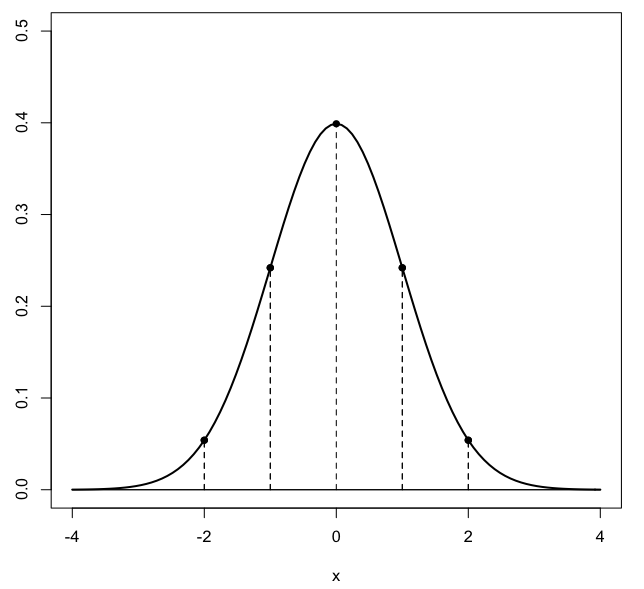
\includegraphics [scale=0.4] {gauss3.png} \end{center}

\title{Hartig and Fitzpatrick}
\date{}

\begin{document}
\maketitle
\Large

This chapter describes two alternative derivations of Kepler's Laws by Hartig and Fitzpatrick. 

The first is from a class handout I found on the web for Math 304 by Hartig.

We start by defining $M$ as the mass of the sun and $m$ as the mass of the planet and $\mathbf{r}$ as the position vector from the sun to the planet.  Combining Newton's second law and the inverse square law of gravitation we have that
\[ \mathbf{F} = m \mathbf{a} = -\frac{GMm}{r^2} \ \frac{\mathbf{r}}{r}  \]
\[ \mathbf{a} = -\frac{GM}{r^2} \ \frac{\mathbf{r}}{r}  \]
We take $\mathbf{u_r}$ as a unit vector in the same direction as $\mathbf{r}$.  I write $\hat{\mathbf{u_r}}$ without its hat ( $\hat{}$ ) as $\mathbf{u_r}$ so as not to confuse it with the derivative $\dot{\mathbf{u}}_\mathbf{r}$.
\[ \mathbf{r} = r \mathbf{u_r} \]
\[ \mathbf{a} = -\frac{GM}{r^2} \ \mathbf{u_r}  \]
The acceleration is along the line of the radial vector, pointing toward the sun.


The velocity is the time-derivative of the position vector $\mathbf{r}$.
\[ \mathbf{v} = \frac{d\mathbf{r}}{dt} = \dot{\mathbf{r}} \]
and the acceleration is
\[ \mathbf{a} = \frac{d\mathbf{v}}{dt} = \ddot{\mathbf{r}} \]

\subsection*{Feynman's dots, again}
We set up the angular momentum as 
\[ \mathbf{L} = \mathbf{r} \times \mathbf{p}  =  \mathbf{r} \times m\mathbf{v}\]
For a unit mass this is
\[ \mathbf{r} \times \mathbf{v} =  \mathbf{r} \times \dot{\mathbf{r}} \]
We compute the time-derivative
\[ \frac{d}{dt} (\mathbf{r} \times \dot{\mathbf{r}}) \]
by the standard vector application of the product rule which we've looked at above, this is equal to 
\[ =  \dot{\mathbf{r}} \times \dot{\mathbf{r}} + \mathbf{r} \times \ddot{\mathbf{r}} \]
and this is equal to zero, since any vector's cross product with itself is zero, including a reversed version of itself, as in the second term.  We define a constant vector $\mathbf{h}$ such that
\[ \mathbf{h} = \mathbf{r} \times \dot{\mathbf{r}} \]
Since $\mathbf{h}$ is a constant, unchanging in both direction and magnitude, it defines a normal vector to the plane containing $\mathbf{r}$ and $\dot{\mathbf{r}}$.  Align $\mathbf{h}$ with the $z$-axis so all the motion occurs in the $xy$-plane.
Note that 
\[ h = |\mathbf{h}| = | \mathbf{r} \times \dot{\mathbf{r}} | = rv \sin \theta \]
where these are all scalar quantities and $\theta$ is the angle between $\mathbf{r}$ and $\dot{\mathbf{r}} = \mathbf{v}$.

\subsection*{Equal area}
We consider the triangle formed by the position vector before and after a short period of time $\Delta t$, and the vector $\Delta \mathbf{r}$ connecting these two positions, where 
\[ \Delta \mathbf{r} \approx \dot{\mathbf{r}} \Delta t \]
The little bit of area $\Delta A$ that is swept out during this time is 
\[ \Delta A \approx \frac{1}{2} \ |\mathbf{r} \times  \dot{\mathbf{r}} \Delta t | \]
\[ \Delta A = \frac{h}{2} \ \Delta t \]
So we have that
\[ \frac{\Delta A}{\Delta t} \approx \frac{h}{2}  \]
and in the limit as $\Delta t \rightarrow 0$
\[ \frac{dA}{dt} = \frac{h}{2}  \]
(Note a difference with Feynman.  He uses $A$ for the area, but never actually computes its value $|\mathbf{r} \times \dot{\mathbf{r}}|$.  Here, $dA/dt$ is the area and it's the second derivative $d^2A/dt^2$ that is equal to zero.  Which is another way of saying that $\mathbf{h}$ is constant).

\subsection*{Manipulating $\mathbf{a} \times \mathbf{h}$}
The crucial step is to prove that
\[ \mathbf{a} \times \mathbf{h} = GM \dot{\mathbf{u}}_\mathbf{r} \]
This takes a bit of work, so I'd like to defer it until the end.  We'll just assume it for now.  Take the equality and integrate with respect to time, obtaining
\[ \int \mathbf{a} \times \mathbf{h} = \int GM \dot{\mathbf{u}}_\mathbf{r} \]
\[ \dot{\mathbf{r}} \times \mathbf{h} = GM \mathbf{u_r} + \mathbf{d} \]
where $\mathbf{d}$ is a constant \emph{vector} of integration.

\subsection*{Dot product}
We're almost there now.  Take the left-hand side from above and form the dot product
\[ \mathbf{r} \cdot (\dot{\mathbf{r}} \times \mathbf{h}) \]
Use another vector identity to switch it around
\[ = (\mathbf{r} \times \dot{\mathbf{r}}) \cdot \mathbf{h} \]
But $\mathbf{r} \times \dot{\mathbf{r}} = \mathbf{h}$ so
\[ = \mathbf{h}  \cdot \mathbf{h} = h^2 \]

\subsection*{conic sections}
What we've shown is that
\[ h^2 = \mathbf{r} \cdot (GM \mathbf{u_r} + \mathbf{d} ) \]
\[ = r(GM + d \cos \theta) \]
\[ = rGM(1 + \frac{d}{GM} \cos \theta ) \]
Define $k = h^2/GM$ and $e = d/GM$.  Then
\[ k = r(1 +e\cos \theta) \]
This is the equation of a conic section.  In particular, if $ e < 1$, then
\[ r = \frac{k}{1 +e\cos \theta} \]
is the equation of an ellipse.  Here is an example with $k=1$ and $e=0.6$
\begin{center} 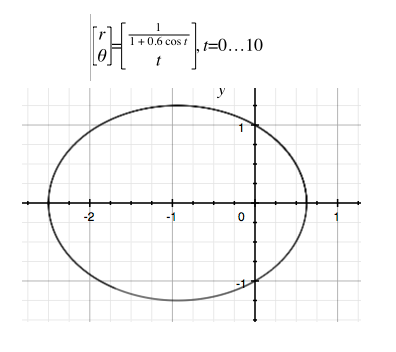
\includegraphics [scale=0.75] {ellipse_param.png} \end{center}

\subsection*{Cleaning up}
Here is a sketch of the situation
\begin{center} 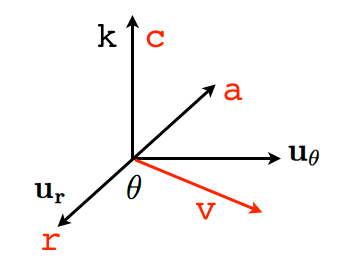
\includegraphics [scale=0.5] {Newton_vecs.png} \end{center}
As we've said all along, $\mathbf{u_r}$ is a unit vector in the $\mathbf{r}$ direction, so that $\mathbf{r} = r \mathbf{u_r}$.  By the central force hypothesis, the acceleration $\mathbf{a} = \dot{\mathbf{v}} = \ddot{\mathbf{r}}$ is in the $- \mathbf{u_r}$ direction.  The source of all our complexity is that $\mathbf{v} = \dot{\mathbf{r}}$ is not perpendicular to $\mathbf{u_r}$ but forms an angle $\theta$ with it.

Also, we defined
\[ \mathbf{h} = \mathbf{r} \times \mathbf{v} \]
and aligned $\mathbf{h}$ with the $\hat{\mathbf{k}}$ direction.  We analyzed $\mathbf{r} \times \mathbf{v}$ to show that $\mathbf{h}$ is a constant vector.
$\mathbf{u_\theta}$ is the unit vector orthogonal to $\mathbf{u_r}$.

According to Hartig, what we have to prove is that
\[ \mathbf{a} \times \mathbf{h} = GM \dot{\mathbf{u}}_\mathbf{r} \]

Go back to basic definitions.
\[ \mathbf{r} = r \mathbf{u_r} \]
\[ \mathbf{v} = \dot{r} \mathbf{u_r} + r \dot{\mathbf{u}}_\mathbf{r} \]
Recall that $\dot{\mathbf{u}}_\mathbf{r} = \dot{\theta} \mathbf{u_\theta}$ so
\[ \mathbf{v} = \dot{r} \mathbf{u_r} + r \dot{\theta} \mathbf{u_\theta} \]
\[ \mathbf{h} = \mathbf{r} \times \mathbf{v} = r \mathbf{u_r} \times (\dot{r} \mathbf{u_r} + r \dot{\theta} \mathbf{u_\theta}) \]
\[ = r^2 \dot{\theta} \hat{\mathbf{k}} \]
The acceleration is
\[ \mathbf{a} = -\frac{GM}{r^2} \mathbf{u}_\mathbf{r} \]
So
\[ \mathbf{a} \times \mathbf{h} = -\frac{GM}{r^2} \mathbf{u}_\mathbf{r} \times r^2 \dot{\theta} \hat{\mathbf{k}} \]
\[ = -GM \dot{\theta} (- \mathbf{u_\theta}) \]
\[= GM \dot{\theta} \mathbf{u_\theta} \]
Again, recall that $\dot{\mathbf{u}}_\mathbf{r} = \dot{\theta} \mathbf{u_\theta}$ so
\[ \mathbf{a} \times \mathbf{h} = GM \dot{\mathbf{u}}_\mathbf{r} \]
Now, integrate
\[ \int \mathbf{a} \times \mathbf{h} = \int GM \dot{\mathbf{u}}_\mathbf{r} \]
\[  \mathbf{v} \times \mathbf{h} = \dot{\mathbf{r}} \times \mathbf{h} =  GM \mathbf{u}_\mathbf{r} \]

\subsection*{Fitzpatrick}

This is a derivation of Kepler's laws from a book I found on the web for Fitzpatrick's course on Mechanics.

He starts by establishing unit vectors in polar coordinates as $\mathbf{e_r}$ and $\mathbf{e_{\theta}}$ and then parametrically
\[ \mathbf{e_r} =  \ \langle \cos \theta, \sin \theta \rangle \]
\[ \mathbf{e_{\theta}} =  \ \langle -\sin \theta, \cos \theta \rangle \]
\[ \mathbf{e_{\theta}} \perp \mathbf{e_r} \]
So
\[ \dot{\mathbf{e}}_\mathbf{r} = \dot{\theta} \mathbf{e_{\theta}} \]
\[ \dot{\mathbf{e}}_\mathbf{\theta} = -\dot{\theta} \mathbf{e_{r}} \]
Writing the position vector as
\[ \mathbf{r} = r \ \mathbf{e_r}  \]
\[ \mathbf{v} = \dot{\mathbf{r}} = \dot{r}\mathbf{e_r} + r \dot{\mathbf{e}}_\mathbf{r} =\dot{r}\mathbf{e_r} + r \dot{\theta} \mathbf{e_{\theta}} \]
For the acceleration
\[ \mathbf{a} = \dot{\mathbf{v}} = \ddot{\mathbf{r}} = \frac{d}{dt} \ (\dot{r}\mathbf{e_r} + r \dot{\theta} \mathbf{e_{\theta}}) \]
 \[ = \ddot{r}\mathbf{e_r} + \dot{r}\dot{\mathbf{e}}_\mathbf{r} + \dot{r} \dot{\theta} \mathbf{e_{\theta}} + r \ddot{\theta} \mathbf{e_{\theta}} + r \dot{\theta}  \dot{\mathbf{e}}_\mathbf{\theta}\]
\[ = \ddot{r}\mathbf{e_r} + \dot{r}\dot{\theta} \mathbf{e_{\theta}} + \dot{r} \dot{\theta} \mathbf{e_{\theta}} + r \ddot{\theta} \mathbf{e_{\theta}} - r \dot{\theta}^2  \mathbf{e}_\mathbf{r}\]
\[ = (\ddot{r} - r \dot{\theta}^2)  \mathbf{e}_\mathbf{r} + (2\dot{r} \dot{\theta} + r \ddot{\theta}) \mathbf{e_{\theta}}  \]
As before we recognize the coefficient for $\mathbf{e_{\theta}}$ as
\[ \frac{1}{r} \frac{d}{dt} (r^2\dot{\theta}) = \frac{1}{r}(2r \dot{r} \dot{\theta} + r^2\ddot{\theta})  \]
and this term is also equal to zero because the acceleration is all radial and so the term in parentheses must be zero and so
\[ 2 r \dot{r} \dot{\theta} + r\ddot{\theta} =  0 \]
if we integrate
\[ \int 2 r \dot{r} \dot{\theta} + r\ddot{\theta} = r^2 \dot{\theta} =  h \]
where $h$ is a constant.

The physical interpretation comes from angular momentum, which is defined as
\[ \mathbf{l} = m \mathbf{r} \times \dot{\mathbf{r}} \]
\[ = m (r \mathbf{e}_\mathbf{r} \times (\dot{r}\mathbf{e_r} + r \dot{\theta} \mathbf{e_{\theta}}) \]
\[ = mr^2  \dot{\theta} \ \hat{\mathbf{k}} \]
That is,
\[ mh \ = | \mathbf{l} | \]
At this point he goes through the standard analysis to obtain that the area swept out in a small time $\delta A/\delta t = h/2$.  I think we can skip this part.


This derivation has an unusual approach to using the information from the inverse square law.  Define a new radial variable, the inverse of $r$
\[ r= \frac{1}{u} \]
Differentiate with respect to time
\[ \dot{r} = - \frac{\dot{u}}{u^2} \]
obviously.  But what is $\dot{u}$?
\[ \dot{u}= \frac{du}{dt} =  \frac{du}{d\theta} \frac{d\theta}{dt} =  \dot{\theta} \ \frac{du}{d\theta} \]
So
\[ \dot{r}= -\frac{1}{u^2} \dot{u} =  -\frac{\dot{\theta}}{u^2} \frac{du}{d\theta} \]
Recall $r^2 \dot{\theta} = \dot{\theta}/u^2 = h$ so
\[ = -h \ \frac{du}{d \theta}\]
Differentiate again with respect to time
\[ \ddot{r} = -h \frac{d}{dt} \ (\frac{du}{d \theta}) = -h \dot{\theta} \ \frac{d^2 u}{d\theta^2} \]
but $\dot{\theta} = hu^2$ so
\[ = - h^2 u^2 \  \frac{d^2 u}{d\theta^2} \]
Now, go back to our previous expression for the acceleration, it is
\[  - \frac{GM}{r^2}  =  \ddot{r} - r \dot{\theta}^2 \]
Plug in for $\ddot{r}$ and multiply everything by $-1$:
\[ \frac{GM}{r^2}  = h^2 u^2 \  \frac{d^2 u}{d\theta^2} + r \dot{\theta}^2 \]
Rearrange ($ru=1$):
\[ \frac{GM}{h^2}  =  \frac{d^2 u}{d\theta^2} + \frac{r^3}{h^2} \dot{\theta}^2 \]
but $h = r^2 \dot{\theta}$ and $h^2 = r^4 \dot{\theta}^2$ so
\[ \frac{GM}{h^2}  =  \frac{d^2 u}{d\theta^2} + \frac{1}{r}  \]
\[ \frac{GM}{h^2}  =  \frac{d^2 u}{d\theta^2} + u \]
How about that?  Now we have a basic differential equation in $u$

We guess the solution has, say $\cos \theta$ and constants $A$ and $C$.
\[ u = A \cos \theta + C \]
because
\[ \frac{d^2 u}{d\theta^2} = -A \cos \theta  \]
So
\[ C = \frac{GM}{h^2} \]
\[ u = A \cos \theta + \frac{GM}{h^2} \]
Technically, we should have $\theta_0$ in the solution, but we can just set that equal to zero, since we don't care about where we start.  Go back to $r$
\[ 1 = r(A \cos \theta + \frac{GM}{h^2}) \]
\[  \frac{h^2}{GM} = r(A \frac{h^2}{GM} + A \cos \theta) \]
Define 
\[ e = A = \frac{GM}{h^2} \]
so now we have
\[ \frac{h^2}{GM} = r(1 + e \cos \theta) \]
which is exactly what we had with Varberg.


\end{document}  